\id{ҒТАМР 65.09.03; 65.09.05}{}

\begin{articleheader}
\sectionwithauthors{М.М. Ташыбаева, А.К. Какимов, Г.А. Жумадилова, А.Б. Бакиева, А.М. Муратбаев}{ОРТАДАН ТЕПКІШ ФОРСУНКА ЖӘНЕ ТІСТІ СОРҒЫ АРҚЫЛЫ ҚОНДЫРҒЫНЫ ЖЕТІЛДІРУ}

{\bfseries
М.М. Ташыбаева\textsuperscript{\envelope },
А.К. Какимов,
Г.А. Жумадилова,
А.Б. Бакиева,
А.М. Муратбаев
}
\end{articleheader}

\begin{affiliation}
«Семей қаласының Шәкәрім атындағы университеті» КеАҚ, Ceмeй, Қазақстан,

\raggedright \textsuperscript{\envelope }Корреспондент-автор: marzhan06081990@gmail.com
\end{affiliation}

Бұл зерттеуде гель түзетін қоспаның тұтқырлығының температура мен натрий
альгинаты ерітіндісінің концентрациясына тәуелділігі зерттелді.40°C
температурада тұтқырлық мәні ротордың айналу жиілігіне аз өзгеретіндігі
анықталып, ерітіндіні пайдалану үшін ең қолайлы температура ретінде
таңдалды. Тісті сорғының 39,3 с⁻¹ және 47,6 с⁻¹ жоғары айналу жиілігінде
қоспаның тұтқырлығы төмендегені байқалды, бұл өз кезегінде форсунка
диаметрлері (0,7×10⁻³ м, 1,0×10⁻³ м, 1,2×10⁻³ м) арқылы өткізгіштік пен
өнімділіктің артуына әкелді. Зерттеу барысында форсунка диаметрінің
капсула өлшемдері мен сапасына әсері анықталды. График бойынша форсунка
тесігінің диаметрі артқан сайын алынған капсулалардың диаметрі де
үлкейетіні байқалды. Диаметрі 0,7×10⁻³ м және 1,0×10⁻³ м болатын
форсункалармен алынған капсулалар пішіні мен құрылымы жағынан талапқа
сай болмады. Ең жақсы нәтиже 1,2×10⁻³ м диаметрлі ортадан тепкіш
форсункада алынды.

Бұл жағдайда капсулалар тұрақты дөңгелек пішінге ие болып, қондырғының
өнімділігін арттыруға мүмкіндік берді. Капсулаларға жүргізілген талдау
нәтижесінде, ең тиімді нұсқа ретінде ортадан тепкіш форсунка диаметрі d
= 1,2×10⁻³ м болатын 3-ші үлгі таңдалып, капсулалауға арналған материал
ретінде 1\% натрий альгинаты қолданылды. Нәтижесінде алынған
капсулалардың орташа диаметрі 1,4×10⁻³ м болды. Қондырғының
энергетикалық сипаттамалары HY4300 мультиметрі арқылы анықталды. Тісті
сорғының әртүрлі айналу жиіліктерінде тұтынатын қуаты өлшенді: 21,4 с⁻¹
-- 28,9 Вт, 30,2 с⁻¹ -- 50,3 Вт, 39,3 с⁻¹ -- 74,8 Вт және 47,6 с⁻¹ --
95,7 Вт. Алынған нәтижелерге сүйене отырып, тұтынылатын қуаттың айналу
жиілігіне тәуелділігін көрсететін график тұрғызылды. Зерттеу нәтижелері
тісті сорғы айналу жиілігі артқан сайын қуат тұтынудың айтарлықтай
өсетінін көрсетті.

{\bfseries Түйін сөздер:} шашырату әдісі, капсула, тісті сорғы, қондырғы,
ортадан тепкіш форсунка, натрий альгинат.

\begin{articleheader}
{\bfseries СОВЕРШЕНСТВОВАНИЕ УСТАНОВКИ С ПОМОЩЬЮ ЦЕНТРОБЕЖНОЙ ФОРСУНКИ И
ШЕСТЕРЕНЧАТОГО НАСОСА}

{\bfseries
М.М. Ташыбаева\textsuperscript{\envelope }
,А.К. Какимов,
Г.А. Жумадилова,
А.Б. Бакиева,
А.М. Муратбаев
}
\end{articleheader}

\begin{affiliation}
НАО «Университет им. Шакарима города Семей», Семей, Казахстан,

e-mail: marzhan06081990@gmail.com
\end{affiliation}

В этом исследовании изучалась зависимость вязкости гелеобразующей смеси
от температуры и концентрации раствора альгината натрия. При 40°C было
обнаружено, что значение вязкости мало изменяется на частоту вращения
ротора, и была выбрана наиболее подходящая температура для использования
раствора. На высоких частотах вращения шестеренчатого насоса 39,3 с⁻¹ и
47,6 с⁻¹ наблюдалось снижение вязкости смеси, что, в свою очередь,
привело к увеличению проводимости и производительности за счет диаметров
форсунки (0,7×10⁻³ м, 1,0×10⁻³ м, 1,2×10⁻³ м). Исследование выявило
влияние диаметра щипцов на размеры и качество капсул. По графику было
замечено, что по мере увеличения диаметра отверстия форсунки
увеличивается и диаметр полученных капсул. Капсулы, полученные щипцами
диаметром 0,7×10⁻³ м и 1,0×10⁻³ м, не соответствовали требованиям по
форме и структуре. Наилучший результат был получен на центробежной
форсунке диаметром 1,2×10⁻³ м. В этом случае капсулы приобрели
устойчивую круглую форму, что позволило повысить производительность
агрегата. В результате проведенного анализа капсул в качестве наиболее
эффективного варианта был выбран 3-й образец с диаметром центробежной
форсунки d = 1,2×10⁻³ м. В качестве материала для капсулирования
использовался 1\% альгинат натрия.

Полученные капсулы имели средний диаметр 1,4×10⁻³ м. Энергетические
характеристики агрегата определялись мультиметром HY4300. Измерена
потребляемая мощность шестеренчатого насоса на различных частотах
вращения: 21,4 с⁻¹ -- 28,9 Вт, 30,2 с⁻¹ -- 50,3 Вт, 39,3 с⁻¹ -- 74,8 Вт
және 47,6 с⁻¹ - 95,7 Вт. На основании полученных результатов построен
график, показывающий зависимость потребляемой мощности от частоты
вращения. Результаты исследования показали, что энергопотребление
значительно увеличивается по мере увеличения частоты вращения
шестеренчатого насоса.

{\bfseries Ключевые слова:} метод распыления, капсула, шестеренчатый насос,
установка, центробежная форсунка, альгинат натрия.

\begin{articleheader}
{\bfseries IMPROVEMENT OF THE INSTALLATION BY MEANS OF A CENTRIFUGAL NOZZLE
AND A GEAR PUMP}

{\bfseries
M.M. Tashybayeva\textsuperscript{\envelope },
А.K. Kakimov,
G.A. Zhumadilova,
A.B. Bakiyeva,
А.M. Muratbayev
}
\end{articleheader}

\begin{affiliation}
NJSC Shakarim University of Semey, Semey, Kazakhstan,

e-mail: marzhan06081990@gmail.com
\end{affiliation}

In this study, the dependence of the viscosity of the gel-forming
mixture on the temperature and \\concentration of the sodium alginate
solution was studied. At 40°C, it was found that the viscosity value
changes little by the rotor speed, and the most suitable temperature for
using the solution was selected. At high rotational speeds of the gear
pump of 39.3 s⁻\textsuperscript{1} and 47.6 s⁻\textsuperscript{1}, a
decrease in the viscosity of the mixture was observed, which, in turn,
led to an increase in conductivity and productivity due to nozzle
diameters (0.7×10\textsuperscript{-3} m, 1.0×10\textsuperscript{-3} m,
1.2×10\textsuperscript{-3} m). The study revealed the influence of the
forceps diameter on the size and quality of the capsules. According to
the graph, it was noticed that as the diameter of the nozzle opening
increases, so does the diameter of the resulting capsules. The capsules
obtained with forceps with a diameter of 0.7×10\textsuperscript{-3} m
and 1.0×10\textsuperscript{-3} m did not meet the shape and structure
requirements. The best result was obtained on a centrifugal nozzle with
a diameter of 1.2×10\textsuperscript{-3} m. In this case, the capsules
acquired a stable round shape, which increased the productivity of the
unit. As a result of the capsule analysis, the 3rd sample with a
diameter of the centrifugal nozzle d = 1.2×10\textsuperscript{-3} m was
chosen as the most effective option.1\% sodium alginate was used as the
encapsulation material. The resulting capsules had an average diameter
of 1.4×10\textsuperscript{-3} m. The energy characteristics of the unit
were determined by a HY4300 multimeter.

The power consumption of a gear pump at various rotational speeds was
measured: 21.4 s⁻\textsuperscript{1} -- 28.9 W, 30.2
s⁻\textsuperscript{1} -- 50.3 W, 39.3 s⁻\textsuperscript{1} -- 74.8 W,
and 47.6 s⁻\textsuperscript{1} - 95.7 W. Based on the results obtained,
a graph is constructed showing the dependence of power consumption on
rotation speed. The results of the study showed that energy consumption
increases significantly as the rotational speed of the gear pump
increases.

{\bfseries Keywords:} spray method, capsule, gear pump, installation,
centrifugal nozzle, sodium alginate.

\begin{multicols}{2}
{\bfseries Кіріспе.} Капсулалау - қорғаныс мембраналары арқылы
ингредиенттерді немесе жасушаларды орау технологиясы. Қорғаныш заттар
(капсулалар) келесі параметрлерге ие болуы керек: жоғары реологиялық
қасиеттер және капсулалау кезінде өңдеу мүмкіндігі, жоғары дисперсиялық
тұрақтылық, капсулаланған затқа инерттілік, жақсы ерігіштік, қол
жетімділігі жатады {[}1{]}. Пробиотиктер жедел ішек инфекцияларында
емдік әсерін тигізеді, ас қорытуды жақсартып қана қоймай жұқпалы
ауруларға төзімділікті арттырады. Адам ағзасына пробиотиктер пайдалы
әсері микроорганизмдер оң қасиеттерімен анықталады. Пробиотиктерді
капсулаға салу, асқазанның қышқыл ортасынан қорғауға көмектеседі,
функционалдық өнімдердің жаңа технологияларына жол ашып береді {[}2,
3{]}. Бұл кезде асқазандағы қышқыл орта капсулаларды 2 сағаттан артық
бұзбауы керек, бірақ капсула ішекке түссе, ол 7 минутта еруі керек {[}4,
5{]}. Капсула ыдыраған кезде ол қажетті пайдалы заттарды шығарады.

Әзірленген капсулалауға арналған жабдықта, тамшылау әдісімен инжектор
фильера көмегімен алынған капсулалар үлкен диаметрлі, өнімділігі аз
болды, құрамында пробиотиктері бар капсулаларды алу процесін
автоматтандыруға мүмкіндік беретін функционалды тамақ өнімдеріне
салынатын капсулаларды алу үшін қондырғыны жетілдіру міндеті қойылды.

Жоғарыда аталған мәселелерді шешу үшін капсулалауға арналған қондырғыны
жетілдіру керек. Мұндай мәселені шешудің оңтайлы жолы, тісті сорғымен
ортадан тепкіш форсунканы қолдану арқылы шашырату әдіспен капсулалауға
арналған қондырғыны жетілдіру болып табылады. Жүргізілген тәжірибелер
және сараптамалар, капсулалау процесінде тісті сорғымен қысым беру
арқылы, шашырату әдіспен ортадан тепкіш форсунканы қолдану арқылы
қондырғыны жетілдіру оңтайлы екенін көрсетті.

Жұмыстың мақсаты ортадан тепкіш форсунка және тісті сорғы арқылы
қондырғыны жетілдіру, шашырату әдіспен капсулалар алу. Мақсатына
байланысты келесідей міндеттер орындалады: капсулалауға арналған
қондырғыны жетілдірудің оңтайлы жолдарын айқындау; қондырғының
құрылымдық параметрлеріне байланысты техникалық сипаттамаларды зерделеу
және жұмыс режимдерін таңдау. Жұмыстың жаңалығы - қондырғының құрылымдық
параметрлеріне байланысты техникалық сипаттамалары зерделеніп және жұмыс
режимдері таңдалды; - алынған капсулалардың тұрақты
құрылымдық-механикалық сипаттамалары мен технологиялық параметрлерін
алуға мүмкіндік беретін ұсынылған ортадан тепкіш форсунка пайдалану
кезінде капсулаларды алудың ұтымды технологиялық режимдері анықталды.

{\bfseries Материалдар мен әдістер.} Гель түзетін қоспаның натрий альгинаты
(0,5\%, 0,8\%, 1\%) концентрациялары таңдалды. Тәжірибе гель түзетін
қоспаның 20 - дан 50 ℃ температурасында жүргізілді, тісті сорғының
айналу жиілігі 21,4 с\textsuperscript{-1}; 30,2 с\textsuperscript{-1};
39,3 с\textsuperscript{-1}; 47,6 с\textsuperscript{-1}; Қондырғыға
форсункалардың оңтайлы диаметрін таңдау үшін 3 (үш) үлгі ортадан тепкіш
форсунка алынды. Форсункадағы тесік диаметрі келесідей: 1 үлгі -- 0,7 ·
10\textsuperscript{-3} м; 2 үлгі -- 1,0· 10\textsuperscript{-3} м; 3
үлгі -- 1,2· 10\textsuperscript{-3} м; 1 -- ші суретте көрсетілген.
Зерттеу жұмысында мынадай әдістер қолданылды: гранулометриялық құрамын
анықтау әдісі, капсула микроқұрылымын анықтау әдістемесі, эксперименттік
қондырғының энергетикалық сипаттамалар әдісі.

Натрий альгинаты гель түзетін қоспа сулы ерітіндісі ретінде алынды.
Ерітінді келесідей алынды: натрий альгинаты 1\% концентрациясы
дайындалды. Натрий альгинаты қоспасы өлшенген стаканда, электромагнитті
қыздырылған араластырғышқа қоямыз және ерітінді толық ерігенше
араластырылады.60 \textsuperscript{о}С қыздыру температурасына қоямыз,
себебі 60 \textsuperscript{о}С - тан төмен температурада натрий
альгинаты нашар ериді, ал 60 \textsuperscript{о}С - тан жоғары
температурада натрий альгинаты жинала бастайды. Натрий альгинаты
ерігеннен қоспасы 40°C температураға дейін салқындатылды. Алынған
қоспаға Propionibacterium freudenreichii пропион қышқылы бактерияларының
штаммы қосылды. Кальций хлоридінің 2\% қалыптау қоспасы дайындалады.
Оған 98 мл тазартылған су алып, 2 грамм кальций хлориді қосамыз. Кальций
хлориді ерітіндісі ерігеннен соң қалып түзетін қоспа дайын болады. Гель
түзетін қоспа тұтқырлығы әр түрлі температурада натрий альгинаты
ерітіндісінің концентрациясына тәуелділігі, 40 және 50 С° температурада
тұтқырлық мөлшері ротордың айналу жиілігі үшін шамалы өзгереді, бірақ
пробиотикалық микроорганизмдердің жойылуын болдырмау үшін 50 С° жоғары
температураны қолданған жөн емес, ерітіндіні пайдаланудың ең қолайлы
температурасы 40 С° алынды {[}6{]}.

Гранулометриялық құрамын анықтау әдісі. Оптикалық микроскопта
зерттелетін объектінің сапалы бейнесін алу үшін жұмысты бастамас бұрын
жарықтандыруды реттеу қажет. Ол үшін сәуле ағынына кішірек үлкейткіш
линзаны (10 немесе одан кіші) және жиналмалы диверсивті линзаны салу
керек. Содан кейін диффузордың тұтқасы толығымен көтеріліп, диффузордың
тесігі толығымен ашылуы керек. Содан кейін объектінің артқы жарығын
қосып, шамның жарықтығын реттеу керек.

Оптикалық микроскоппен бақылаулар мен зерттеулер жүргізгенде, бүйірлік
жарықтың, әсіресе қуатты окулярлармен жұмыс істегенде айтарлықтай
кедергі тудыруы мүмкін екенін ескеру қажет. Капсула графикалық қағазда 2
- суретте көрсетілген. Үстел үстіндегі заттың сапалы бейнесін алу үшін
микроскопты сәулелену көзі ретінде экранға бөгде заттардың түсуін
болдырмайтындай етіп бағыттау керек {[}7{]}.
\end{multicols}

\begin{figure}[H]
	\centering
	\begin{subfigure}[b]{0.32\textwidth}
		\centering
		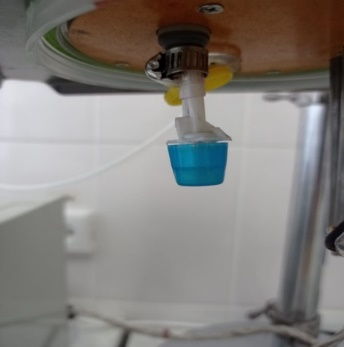
\includegraphics[width=\textwidth,height=\textwidth]{media/pish/image20}
		\caption*{d= 0,7×10\textsuperscript{-3}м}
	\end{subfigure}
	\hfill
	\begin{subfigure}[b]{0.32\textwidth}
		\centering
		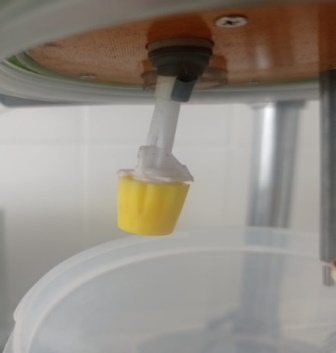
\includegraphics[width=\textwidth,height=\textwidth]{media/pish/image21}
		\caption*{d= 1,0×10\textsuperscript{-3}м}
	\end{subfigure}
	\hfill
	\begin{subfigure}[b]{0.32\textwidth}
		\centering
		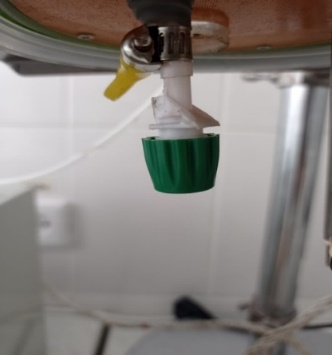
\includegraphics[width=\textwidth,height=\textwidth]{media/pish/image22}
		\caption*{d= 1,2×10\textsuperscript{-3}м}
	\end{subfigure}
	\caption*{\bfseries 1 - сурет. Ортадан тепкіш форсункалар түрлері}
\end{figure}

\begin{figure}[H]
	\centering
	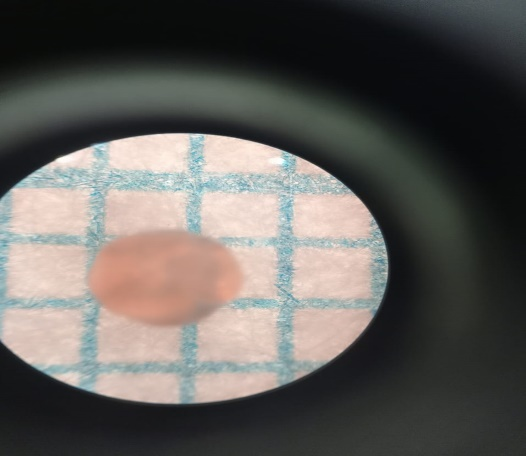
\includegraphics[width=0.32\textwidth]{media/pish/image23}
	\caption*{2 - сурет. Гранулометриялық құрамын анықтау әдісі}
\end{figure}

\begin{multicols}{2}
Үлкейтуі X10 - нан асатын линзаларды пайдаланған кезде конденсатордың
жиналмалы линзасын арқалықтардан алып тастап, окулярды салу керек. Егер
жарықтандырылған өрістің жарықтығын азайту немесе объектінің контрастын
өзгерту қажет болса, оны конденсатордың жиналмалы жақтауына орнату
арқылы жарық сүзгісін қолдануға болады. Капсуланың шамамен радиусы
миллиметрлік қағаз торының көмегімен есептелді және
1,4·10\textsuperscript{-3} м болды.

Капсула микроқұрылымын анықтау әдістемесі. Саңылаулардың геометриялық
өлшемдерін өлшеу үшін рентген жүйесі бар JEOL (Жапония) фирмасының
«JSM-6390LV» төмен вакуумды аналитикалық сканерлеуші электронды
микроскопы (SEM) пайдаланылды {[}8, 9{]}. «OXFORD INSTRUMENTS»
(Ұлыбритания) компаниясының «INCA ENERGY 250» микроанализаторы. Бұл
микроскоп зерттелетін үлгінің химиялық құрамын 0,1\% дәлдікпен анықтауға
және картаға түсіруге мүмкіндік береді, материалдың құрылымын жоғары
және төмен вакуумдық режимдерде 30 - дан 300 000 есеге дейін үлкейтеді
{[}10{]}. JEOL (Жапония) JFD-320 терт-бутил спиртін қолданып мұздатып
кептіру кезінде вакуумның әсерінен мұздатылған күйден бу күйіне бірден
ауысады. Бұл капсуладан терт-бутил спиртін шығаруға мүмкіндік береді
және оның құрылымын сақтайды. Содан кейін JEOL (Жапония) шығарған JEE -
420 вакуумды шашыратқыш машинада капсула тілімінің бетіне көміртегі
қабаты жағылады, бұл контрастты жоғарырақ кескіндерді алуға мүмкіндік
береді. Дайындалған капсулалар екі жақты көміртекті таспаның көмегімен
бекітіледі. Содан кейін оны микроскоп камерасына салып, беттерін
сканерлейді {[}11, 12{]}.

Эксперименттік қондырғының энергетикалық сипаттамалар әдісі.3 - суретте
қолданылатын құрылғылар тұрақты токты 5 - тен 200 вольтке дейін ауыстыру
үшін қатты реле қажет етіп жасалған, ток күші 40 амперге дейін. Басқару
кернеуі 3-тен 32 вольтке дейін. Ал тармақтардағы ток күшін, кернеуді
шектеу, реттеу үшін айнымалы сымды резисторлар тізбегі қолданылады.
\end{multicols}

\begin{figure}[H]
	\centering
	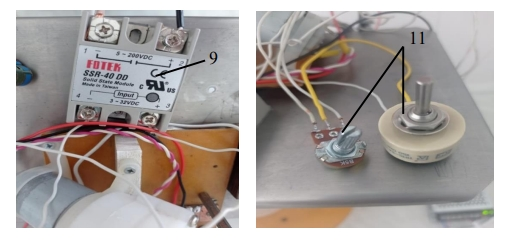
\includegraphics[width=0.6\textwidth]{media/pish/image24}
	\caption*{3 - сурет. Қатты күйдегі реле және резисторлар}
\end{figure}
\begin{figure}[H]
	\centering
	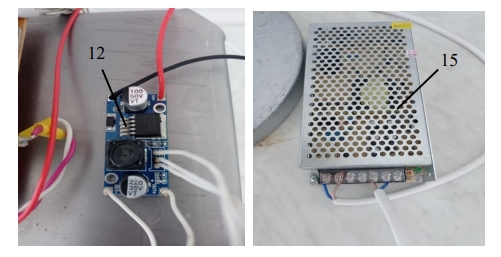
\includegraphics[width=0.6\textwidth]{media/pish/image25}
	\caption*{4 - сурет. Тұрақты кернеуді төмендететін тұрақтандырғыш және қуат көзі}
\end{figure}

\begin{multicols}{2}
4 - суреттегі тұрақты кернеу тұрақтандырғышы - бұл электр жүйесінде
тұрақты кернеу деңгейін ұстап тұру үшін қолданылатын құрылғы. Тұрақты
кернеу тұрақтандырғышының мақсаты - желідегі кернеудің ауытқуын өтеу
және тұрақты шығыс кернеуін қамтамасыз ету. Қуат көзі - бұл құрылғыны
қуаттандыру үшін электр қуатын беретін және реттейтін электрондық
құрылғы. Әрі қарай, гель түзетін қоспаның сулы ерітіндісі жүйенің тиеу
бункеріне жүктеліп, капсулалар шығарылды. Ток күшін, кернеуді өлшеу үшін
смартфон камерасы арқылы құрылғылардағы электр шамаларының сәйкес
мәндері жазылды. Осыдан кейін өлшеу нәтижелері алынған бейнеден
кезең-кезеңімен оқылды.

{\bfseries Нәтижелер және талқылау.} Микроқұрылымды анықтау және
капсулалардың геометриялық өлшемдерін өлшеу. Натрий альгинаты 0,5\%,
0,8\%, 1\% ерітіндісінен алынған капсулалар 5 - 7 суреттерде
көрсетілгендей.
\end{multicols}

\begin{figure}[H]
	\centering
	\begin{subfigure}[b]{0.3\textwidth}
		\centering
		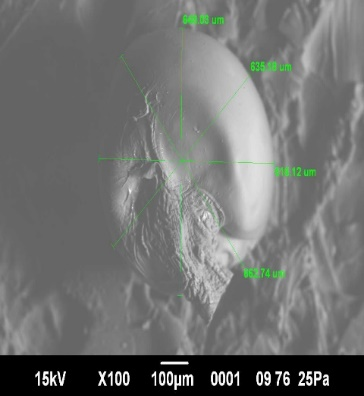
\includegraphics[height=5cm,width=5cm]{media/pish/image26}
		\caption*{0,5\% натрий альгинат}
	\end{subfigure}
	\hfill
	\begin{subfigure}[b]{0.3\textwidth}
		\centering
		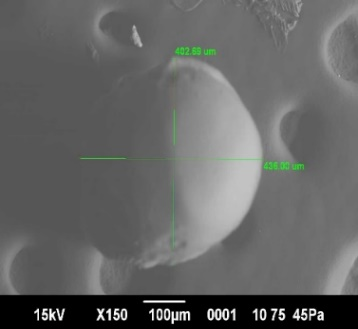
\includegraphics[height=5cm,width=5cm]{media/pish/image27}
		\caption*{0,8 \% натрий альгинат}
	\end{subfigure}
	\hfill
	\begin{subfigure}[b]{0.3\textwidth}
		\centering
		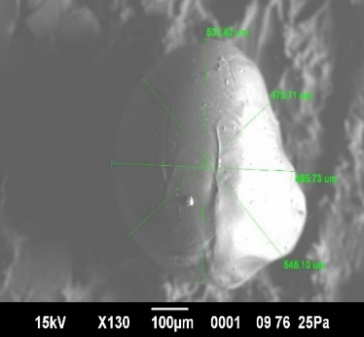
\includegraphics[height=5cm,width=5cm]{media/pish/image28}
		\caption*{1 \% натрий альгинат}
	\end{subfigure}
	\caption*{5 - сурет. Микроскоптау нәтижелері 0,7×10\textsuperscript{-3}м алынған капсулалар}
\end{figure}

\begin{figure}[H]
	\centering
	\begin{subfigure}[b]{0.3\textwidth}
		\centering
		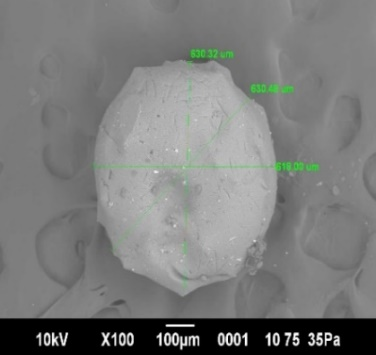
\includegraphics[width=5cm,height=5cm]{media/pish/image29}
		\caption*{0,5\% натрий альгинат}
	\end{subfigure}
	\hfill
	\begin{subfigure}[b]{0.3\textwidth}
		\centering
		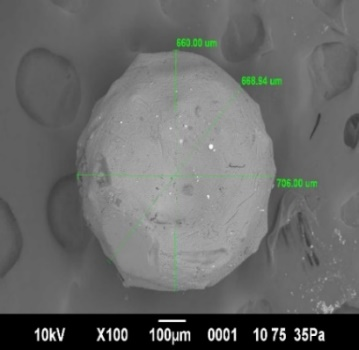
\includegraphics[width=5cm,height=5cm]{media/pish/image30}
		\caption*{0,8 \% натрий альгинат}
	\end{subfigure}
	\hfill
	\begin{subfigure}[b]{0.3\textwidth}
		\centering
		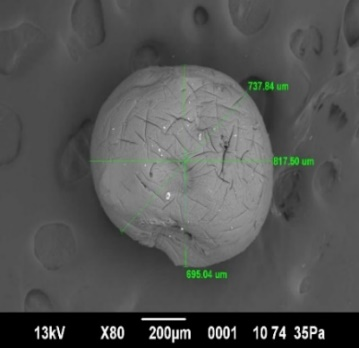
\includegraphics[width=5cm,height=5cm]{media/pish/image31}
		\caption*{1 \% натрий альгинат}
	\end{subfigure}
	\caption*{6 - сурет. Микроскоптау нәтижелері 1,0×10\textsuperscript{-3}м алынған капсулалар}
\end{figure}

\begin{figure}[H]
	\centering
	\begin{subfigure}[b]{0.3\textwidth}
		\centering
		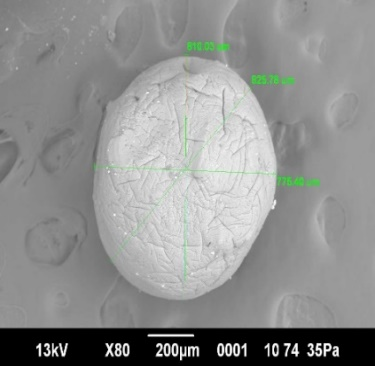
\includegraphics[width=5cm,height=5cm]{media/pish/image32}
		\caption*{0,5\% натрий альгинат}
	\end{subfigure}
	\hfill
	\begin{subfigure}[b]{0.3\textwidth}
		\centering
		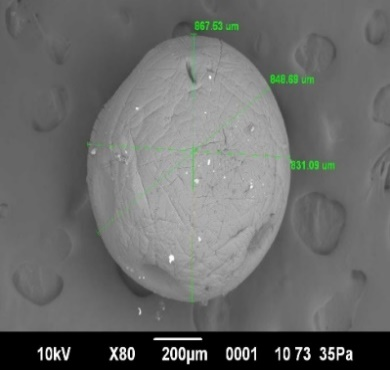
\includegraphics[width=5cm,height=5cm]{media/pish/image33}
		\caption*{0,8 \% натрий альгинат}
	\end{subfigure}
	\hfill
	\begin{subfigure}[b]{0.3\textwidth}
		\centering
		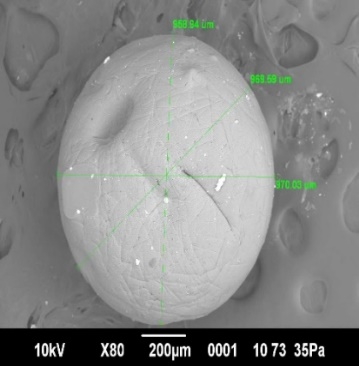
\includegraphics[width=5cm,height=5cm]{media/pish/image34}
		\caption*{1 \% натрий альгинат}
	\end{subfigure}
	\caption*{7 - сурет. Микроскоптау нәтижелері 1,2×10\textsuperscript{-3}м алынған капсулалар}
\end{figure}

Тәжірибе жасау кезінде 1 үлгідегі форсунка тесік диаметрі
d=0,7×10\textsuperscript{-3}м, натрий алгинатының концентрациясы 0,5\%
капсуладағы тұтқырлығы төмен болды, 8 - суретте капсулалар дұрыс емес
пішінді және дұрыс емес құрылымды болды, жұмсақ консистенциялы,
физикалық әсерден оңай бұзылады, орташа диаметрі
0,4×10\textsuperscript{-3}м болды. Ал натрий альгинаты 0,8\%
концентрациясында алынған капсулалар пішіні дұрыс емес және құрылымы
дұрыс емес, консистенциясы жұмсақ, физикалық әсерден оңай бұзылатын,
орташа диаметрі 0,6×10\textsuperscript{-3}м. Натрий альгинаты 1\%
концентрациясында алынған капсулалар пішіні дөңгелек шар тәрізді және
біркелкі, жұмсақ, бірақ физикалық әсерге тұрақты диаметрі
0,7×10\textsuperscript{-3}м болды.

\begin{figure}[H]
	\centering
	\begin{subfigure}[b]{0.3\textwidth}
		\centering
		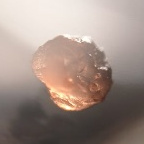
\includegraphics[width=5cm,height=5cm]{media/pish/image35}
		\caption*{0,5\% натрий альгинаты}
	\end{subfigure}
	\hfill
	\begin{subfigure}[b]{0.3\textwidth}
		\centering
		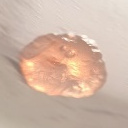
\includegraphics[width=5cm,height=5cm]{media/pish/image36}
		\caption*{0,8\% натрий альгинаты}
	\end{subfigure}
	\hfill
	\begin{subfigure}[b]{0.3\textwidth}
		\centering
		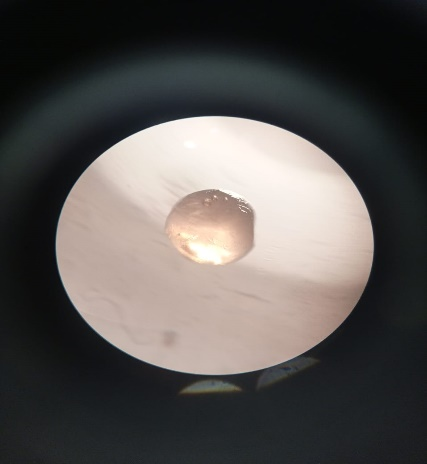
\includegraphics[width=5cm,height=5cm]{media/pish/image37}
		\caption*{1\% натрий альгинаты}
	\end{subfigure}
	\caption*{8 - сурет. Микроскоптау нәтижелері алынған d=0,7×10\textsuperscript{-3}м капсулалар}
\end{figure}

Форсунка тесігінің диаметрі 2 үлгідегі d=1,0×10\textsuperscript{-3}м,
0,5\% натрий альгинаты концентрациясында алынған капсула 9 - суретте
көрсетілгендей пішіні дұрыс емес және құрылымы дұрыс емес,
консистенциясы жұмсақ, физикалық әсерден оңай бұзылады, орташа диаметрі
0,9×10\textsuperscript{-3}м болады.

\begin{figure}[H]
	\centering
	\begin{subfigure}[b]{0.3\textwidth}
		\centering
		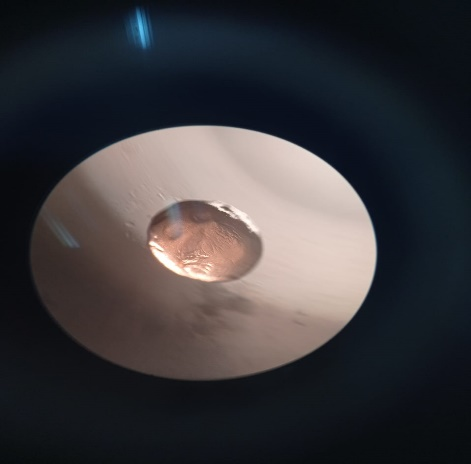
\includegraphics[width=5cm,height=5cm]{media/pish/image38}
		\caption*{0,5\% натрий альгинаты}
	\end{subfigure}
	\hfill
	\begin{subfigure}[b]{0.3\textwidth}
		\centering
		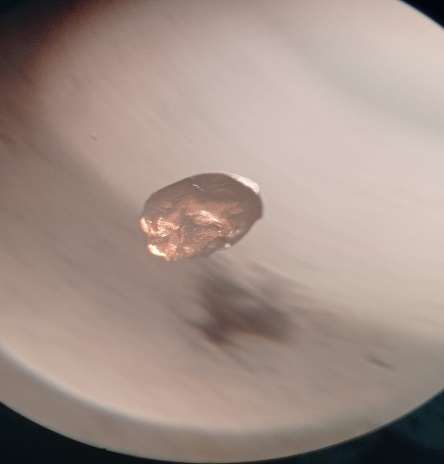
\includegraphics[width=5cm,height=5cm]{media/pish/image39}
		\caption*{0,8\% натрий альгинаты}
	\end{subfigure}
	\hfill
	\begin{subfigure}[b]{0.3\textwidth}
		\centering
		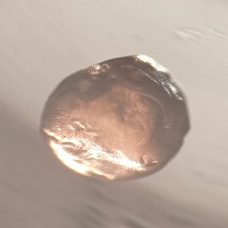
\includegraphics[width=5cm,height=5cm]{media/pish/image40}
		\caption*{1\% натрий альгинаты}
	\end{subfigure}
	\caption*{9 - сурет. Микроскоптау нәтижелері алынған d=1,0×10\textsuperscript{-3}м капсулалар}
\end{figure}

Ал 0,8\% натрий альгинаты концентрациясында пішіні дұрыс емес құрылымды
капсулалар жұмсақ консистенцияға ие, физикалық әсерден оңай бұзылады
және орташа диаметрі 1,1×10\textsuperscript{-3}м болды.1\% натрий
алгинаты концентрациясында алынған капсулалар дөңгелек пішінді және
біркелкі, жұмсақ, бірақ физикалық әсерде тұрақты және орташа диаметрі
1,2×10\textsuperscript{-3}м болды {[}13, 14{]}.

Сонымен, форсунка тесігінің диаметрі 3 үлгідегі тәжірибеде
d=1,2×10\textsuperscript{-3}м үлгідегі 0,5\% натрий алгинаты капсулалары
концентрациясында алынған капсулалар 10 - суретте көрсетілгендей пішіні
біркелкі және құрылымы біртекті, консистенциясы жұмсақ болды, физикалық
әсерден оңай бұзылады, орташа диаметрі 1,1×10\textsuperscript{-3}м
болды.

\begin{figure}[H]
	\centering
	\begin{subfigure}[b]{0.3\textwidth}
		\centering
		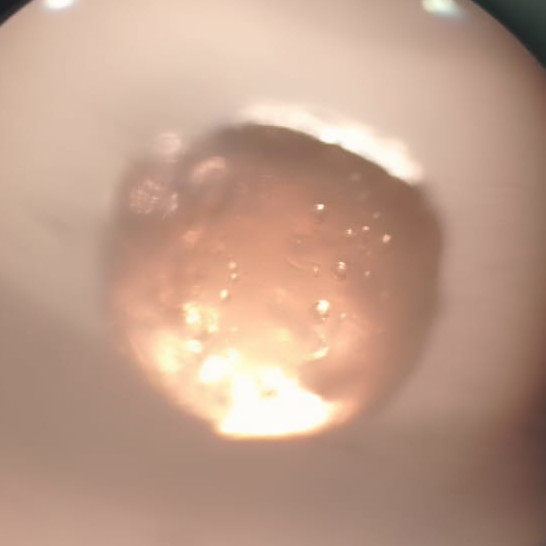
\includegraphics[width=5cm,height=5cm]{media/pish/image41}
		\caption*{0,5\% натрий альгинаты}
	\end{subfigure}
	\hfill
	\begin{subfigure}[b]{0.3\textwidth}
		\centering
		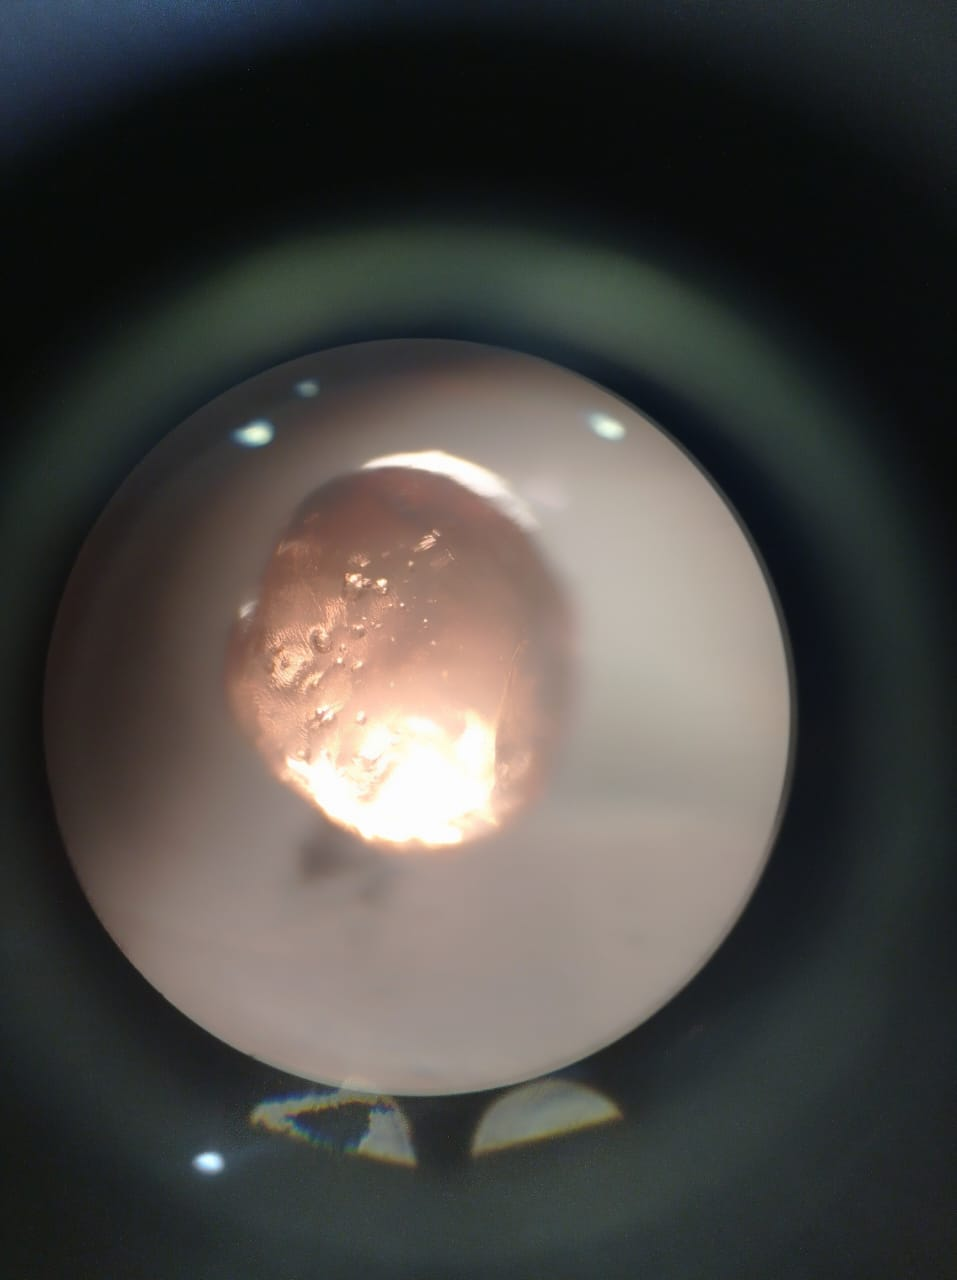
\includegraphics[width=5cm,height=5cm]{media/pish/image42}
		\caption*{0,8\% натрий альгинаты}
	\end{subfigure}
	\hfill
	\begin{subfigure}[b]{0.3\textwidth}
		\centering
		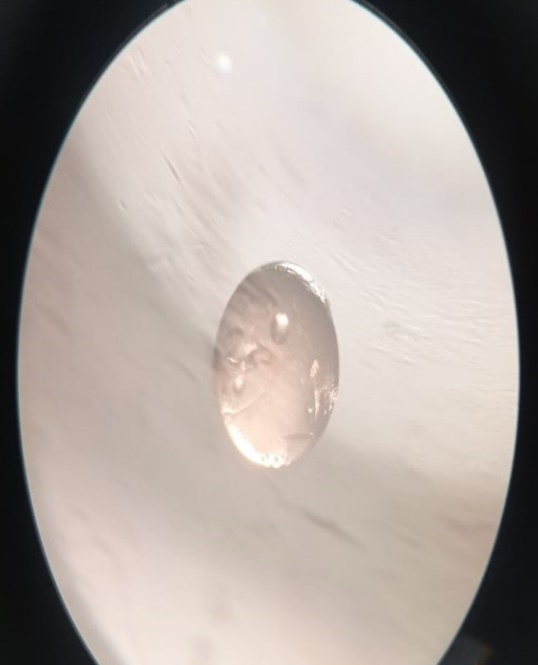
\includegraphics[width=5cm,height=5cm]{media/pish/image43}
		\caption*{1\% натрий альгинаты}
	\end{subfigure}
	\caption*{10 - сурет. Микроскоптау нәтижелері алынған d=1,2×10\textsuperscript{-3}м капсулалар}
\end{figure}

\begin{multicols}{2}
Ал 0,8\% натрий алгинаты концентрациясында алынған капсулалар қалыпты
пішінді және біртекті консистенциялы, физикалық әсерден оңай бұзылады,
орташа диаметрі 1,3×10\textsuperscript{-3}м болады.1\% альгинат
концентрациясында жоғары тұтқырлыққа байланысты алынған капсулалар
дөңгелек пішінді және біртекті, жұмсақ, физикалық әсер кезінде тұрақты,
орташа диаметрі 1,4×10\textsuperscript{-3}м болды {[}15{]}.

Капсулаларға талдау жүргізе отырып, оңтайлы деп 3 үлгі ортадан тепкіш
форсунка тесік диаметрі d=1,2×10\textsuperscript{-3}м алынды, ал
капсулалауға арналған материал ретінде 1\% натрий альгинаты
концентрациясы қабылданды, себебі алынған капсулалар талаптарға сәйкес
келеді, алынған капсула орташа диаметрі 1,4×10\textsuperscript{-3}м
болды. Осы құрамнан жасалған капсулалар әдемі дөңгелек пішінді, құрылымы
біркелкі, жұмсақ консистенциялы, физикалық әсерге төзімді болып келеді.

Капсула өлшемдерінің ортадан тепкіш форсунка тесіктерінің диаметріне
тәуелділігін анықтау үшін 11 - суретте графикте көрсетілген. Графикте
форсунка диаметрінің капсула өлшемдеріне әсері көрсетілген, ал тәжірибе
жүргізу кезінде форсунка тесіктерінің диаметрі үлкейген сайын, алынған
капсулалар диаметрі де үлкейді.
\end{multicols}

\begin{figure}[H]
	\centering
	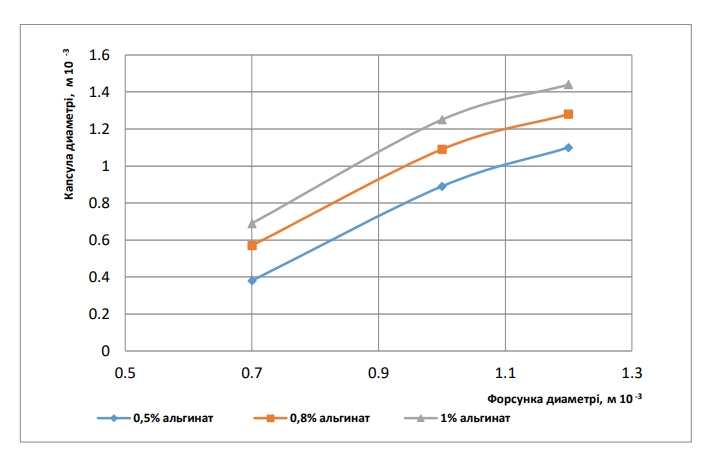
\includegraphics[width=0.7\textwidth]{media/pish/image44}
	\caption*{11 - сурет. Капсула диаметрінің форсункадағы тесік диаметріне тәуелділігі}
\end{figure}

Әр түрлі пайдаланылған ортадан тепкіш форсункалар арқылы, тісті сорғының
айналу жиілігіне байланысты, қондырғының өнімділігі анықталды, 12 -- ші
суретте көрсетілгендей.

\begin{figure}[H]
	\centering
	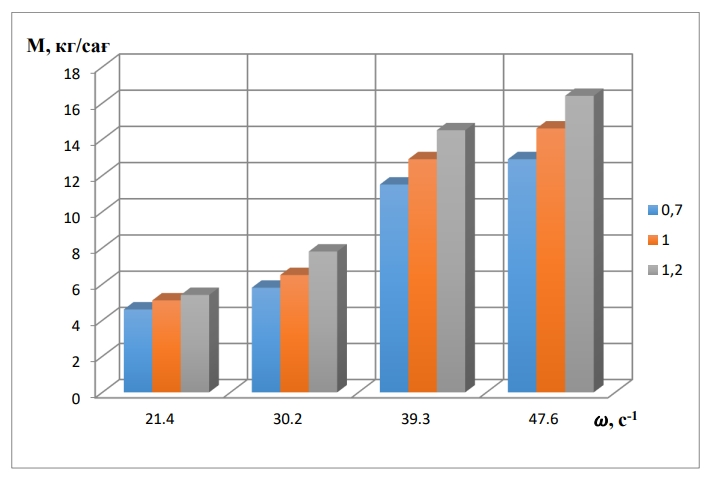
\includegraphics[width=0.7\textwidth]{media/pish/image45}
	\caption*{12 - сурет. Қондырғы өнімділігі пайдаланылатын форсунка түріне тәуелділігі}
\end{figure}

\begin{figure}[H]
	\centering
	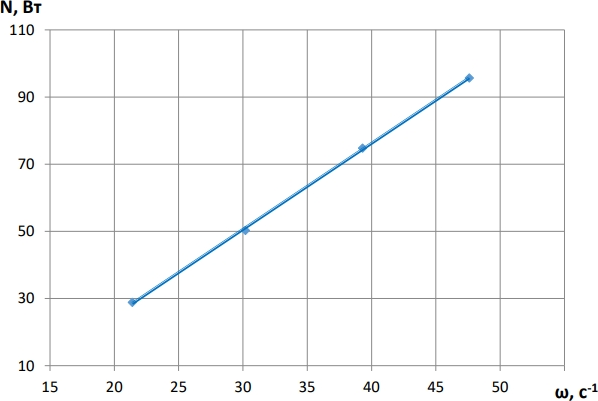
\includegraphics[width=0.7\textwidth]{media/pish/image46}
	\caption*{13 - сурет. Қондырғының тұтынылатын қуаты}
\end{figure}

\begin{multicols}{2}
Тісті сорғының айналу жиілігінің өсуімен, қондырғының тұтынылатын қуаты
да өсетін көруге болады. HY4300 мультиметрінде қондырғының энергетикалық
сипаттамаларын анықталды, 13 - суретке сәйкес график тұрғызылды.

Төмен айналу жиілігінде 21,4 с\textsuperscript{-1}, 30,2
с\textsuperscript{-1} тісті сорғының форсунка диаметрлері
0,7×10\textsuperscript{-3}м, 1,0×10\textsuperscript{-3}м,
1,2×10\textsuperscript{-3}м өнімділігі аз болады, себебі Ньютондық емес
сұйықтық болып табылады. Төмен жылдамдықта гель түзетін қоспа тұтқырлығы
жоғары болады, нәтижесінде диаметрі үлкен форсунканың өткізу қабілеті
жоғары болады. Жоғары айналу жиілігінде тісті сорғының 39,3
с\textsuperscript{-1}, 47,6 с\textsuperscript{-1} гель түзетін қоспаның
тұтқырлығы төмендейді, 0,7×10\textsuperscript{-3}м,
1,0×10\textsuperscript{-3}м, 1,2×10\textsuperscript{-3}м форсунка
диаметрлері өткізу қабілеті өнімділігі артады {[}16, 17{]}.

{\bfseries Қорытынды.} Тұтқырлық пен температураның байланысы натрий
альгинаты ерітіндісінің концентрациясы мен температураға тәуелділігі
зерттелген.40°C температурасы ең қолайлы ретінде таңдалған, себебі бұл
температурада тұтқырлық ротор айналу жиілігіне аз тәуелді. Капсулалау
параметрлері ортадан тепкіш форсунка тесігінің диаметрі:
d=1,2×10\textsuperscript{-3} м, капсулалау материалы: 1\% натрий
альгинаты ерітіндісі. Алынған капсулалардың орташа диаметрі:
1,4×10\textsuperscript{-3}м. Бұл зерттеудің негізгі нәтижелері өндіріс
процесін тұрақтандыруға және капсула сапасын жақсартуға көмектеседі.
\end{multicols}

\begin{center}
{\bfseries Әдебиеттер}
\end{center}

\begin{references}
1. Тихонов С.Л., Харапаев М.Н., Тихонова Н.В. Микрокапсулирование
аскорбиновой кислоты и его использование в пищевой промышленности //
е-forum. - 2020. - № 3 (12). - 13 с.

2. Нуpбeкoвa Г.Б., Бaйбaлинoвa Г.М., Кaкимoвa Ж.Х. Oбщaя хapaктepиcтикa
и биoлoгичecкaя poль пpoбиoтикoв // Вecтник ГУ им. Шaкapимa.- 2015. - №1
(69). -- C.29-31.

3. Бепеева А.Е. Иccлeдoвaниe и paзpaбoткa тeхнoлoгии пpoизвoдcтвa
киcлoмoлoчнoгo пpoдуктa c инкaпcулиpoвaнными пpoбиoтикaми диc. ... д-pa
филocoфии (PhD): 6D072700 - Тeхнoлoгия пpoдoвoльcтвeнных пpoдуктoв.-
Семей: ГУ им. Шaкapимa, Ceмeй, 2016. -- 167с

4. Saad N., Delattre C., Urdaci M., Schmitter J.M., Bressollier P. An
overview of the last advances in probiotic and prebiotic field // LWT -
Food Science and Technology. - 2013.-Vol.50(1). -- Р.1-16. DOI
10.1016/j.lwt.2012.05.014

5. Ran S., Xiao-Li Zh., Dai-Di F., Yu M., Chan-Yuan Y., Xin J.
Encapsulation of probiotic Bifidobacterium longum BIOMA 5920 with
alginate-- human-like collagen and evaluation of survival in simulated\\
gastrointestinal conditions// International Journal of Biological
Macromolecules. - 2011.- Vol.49(5). - P.979-984.
DOI~

6. ҚР пайдалы модельге патенті № 9093. Капсулаған өнімдерді өндіруге
арналған қондырғы. Ташыбаева М.М., Какимов А.К., Майоров А.А., Ибрагимов
Н.К., Джумажанова М.М., Жумадилова Г.А., Муратбаев А.М., Бакиева А.Б.,
Дукенбаев Д.К.

7. Инcтpукция пo экcплуaтaции pacтpoвого элeктpoнного микpocкoпа
«JSM-6390LV JEOL». -- Япoния, 2008.- 42 с.

8. Дюсембаев С.Т., Ибрагимов Н.К., Иминова Д.Е., Омаргалиева Н.К.,
Бедьярова С.К. Методика приготовления препаратов растений для растрового
электронного микроскопа // Мат. межд. научно-практ. конф. «Перспективы
инновационного развития АПК в Казахстане».- Семей, 2014. - С.142-144

9. Joseph I.G., Dale E.N., Echlin P., David C., Joy C., Fiori E. Lifshin
Scsnning Electron Microscopy and X-Ray Microanalysis.- New York, General
Electric Corporate, 1989. - 673 p.

~ISBN 978-1-4613-4969-3, ISBN 978-1-4615-0215-9 (eBook)

10. Piz D. Histological technique in electron microscopy: Electron
Microscopy // Interscience.- New York, 2013. -160 p.ISBN 9781483231921

11. Техническое описание и инструкция по эксплуатации замораживающий
столик ОЛ-30 -- Харьков: Завод-производитель ООО Индмедпром, 2010.- 12
с.

12. Техническое описание и инструкция по эксплуатации Микротом санный
МС-2 -- Харьков: Издательство «ПРАПОР», 2010.- 10 с.

13. Инcтpукция пo экcплуaтaции лиофильную сушку JFD-320 JEOL. -- Япoния,
2009. - 10 с.

14. Инcтpукция пo экcплуaтaции вакуумной напыляющей установки JEE-420
JEOL. -- Япoния, 2010.- 14 с.

15. Ташыбаева М.М. Тамақ өнімдерін капсулалауға арналған қондырғыны
жетілдіру. - Семей: «Семей қаласының Шәкәрім атындағы университеті»
КеАҚ, 2024. -- 114 б.
\href{https://shakarim.edu.kz/upload/editor/pages/science/dissertation/Tashybaeva/kaz-1.pdf}{}

16. Tashybayevа М., Kakimov A., Ibragimov N., Zhumadilova G., Muratbayev
A., Jumazhanova M., Idyryshev B., Kapshakbayeva Z ., Bepeyeva A.
Optimization of encapsulation parameters for sodium alginate capsules: A
study on the effect of temperature and gear pump rotation speed on
capsule production and quality // Food Process Engineering. -- 2024. -
№47(7):e14687. 

17. Ташыбаева М.М., Какимов А.К., Майоров А.А., Жумадилова Г.А.
Установка для капсулирования пробиотиков // Вестник КазУТБ. -- Астана.
-- 2024. - №3(24). -- С.399-410.
\href{https://doi.org/10.58805/kazutb.v.3.24-353}{}
\end{references}

\begin{center}
{\bfseries References}
\end{center}

\begin{references}
1. Tihonov S.L., Harapaev M.N., Tihonova N.V. Mikrokapsulirovanie
askorbinovoj kisloty i ego ispol' zovanie v pishhevoj
promyshlennosti // e-forum. - 2020. - № 3 (12). - 13 s. {[}in Russian{]}

2. Nupbekova G.B., Bajbalinova G.M., Kakimova Zh.H. Obshhaja
hapaktepictika i biologicheckaja pol'{} ppobiotikov //
Vectnik GU im. Shakapima.- 2015. - №1 (69). -- C.29-31. {[}in
Russian{]}

3. Bepeeva A.E. Iccledovanie i pazpabotka tehnologii ppoizvodctva
kiclomolochnogo ppodukta c \\inkapculipovannymi ppobiotikami dic. ... d-pa
filocofii (PhD): 6D072700 - Tehnologija podovol' ctvennyh
ppoduktov.- Semej: GU im. Shakapima, Cemej, 2016. -167s. {[}in
Russian{]}

4. Saad N., Delattre C., Urdaci M., Schmitter J.M., Bressollier P. An
overview of the last advances in probiotic and prebiotic field // LWT -
Food Science and Technology. - 2013.-Vol.50(1). -- Р.1-16. DOI
10.1016/j.lwt.2012.05.014

5. Ran S., Xiao-Li Zh., Dai-Di F., Yu M., Chan-Yuan Y., Xin J.
Encapsulation of probiotic Bifidobacterium longum BIOMA 5920 with
alginate-- human-like collagen and evaluation of survival in simulated\\
gastrointestinal conditions// International Journal of Biological
Macromolecules. - 2011.- Vol.49(5). - P.979-984. DOI

6. ҚR pajdaly model' ge patentі № 9093. Kapsulaғan
өnіmderdі өndіruge arnalғan қondyrғy. Tashybaeva M.M., Kakimov A.K.,
Majorov A.A., Ibragimov N.K., Dzhumazhanova M.M., Zhumadilova G.A.,\\
Muratbaev A.M., Bakieva A.B., Dukenbaev D.K.{[}in Kazakh{]}

7. Inctpukcija po jekcpluatacii pactpovogo jelektponnogo mikpockopa
«JSM-6390LV JEOL». -- Japonija, 2008.- 42 s. {[}in Russian{]}

8. Djusembaev S.T., Ibragimov N.K., Iminova D.E., Omargalieva N.K.,
Bed' jarova S.K. Metodika \\prigotovlenija preparatov
rastenij dlja rastrovogo jelektronnogo mikroskopa // Mat. mezhd.
nauchno-prakt. konf. «Perspektivy innovacionnogo razvitija APK v
Kazahstane».- Semej, 2014. - S.142-144. {[}in Russian{]}

9. Joseph I.G., Dale E.N., Echlin P., David C., Joy C., Fiori E. Lifshin
Scsnning Electron Microscopy and X-Ray Microanalysis.- New York, General
Electric Corporate, 1989. - 673 p.

ISBN 978-1-4613-4969-3, ISBN 978-1-4615-0215-9 (eBook)

10. Piz D. Histological technique in electron microscopy: Electron
Microscopy // Interscience.- New York, 2013. -160 p.ISBN 9781483231921

11. Техническое описание и инструкция по эксплуатации замораживающий
столик ОЛ-30 -- Харьков: Завод-производитель ООО Индмедпром, 2010.- 12
с. {[}in Russian{]}

12. Техническое описание и инструкция по эксплуатации Микротом санный
МС-2 -- Харьков: Издательство «ПРАПОР», 2010.- 10 с. {[}in Russian{]}

13. Инcтpукция пo экcплуaтaции лиофильную сушку JFD-320 JEOL. -- Япoния,
2009. - 10 с.

14. Инcтpукция пo экcплуaтaции вакуумной напыляющей установки JEE-420
JEOL. -- Япoния, 2010.- 14 с. {[}in Russian{]}

15. Ташыбаева М.М. Тамақ өнімдерін капсулалауға арналған қондырғыны
жетілдіру. - Семей: «Семей қаласының Шәкәрім атындағы университеті»
КеАҚ, 2024. -- 114 б.
\href{https://shakarim.edu.kz/upload/editor/pages/science/dissertation/Tashybaeva/kaz-1.pdf}{https://shakarim.edu.kz}
{[}in Kazakh{]}

16. Tashybayevа М., Kakimov A., Ibragimov N., Zhumadilova G., Muratbayev
A., Jumazhanova M., Idyryshev B., Kapshakbayeva Z ., Bepeyeva A.
Optimization of encapsulation parameters for sodium alginate capsules: A
study on the effect of temperature and gear pump rotation speed on
capsule production and quality // Food Process Engineering. -- 2024. -
№47(7):e14687. 

17. Tashybaeva M.M., Kakimov A.K., Majorov A.A., Zhumadilova G.A.
Ustanovka dlja kapsulirovanija probiotikov // Vestnik KazUTB. -- Astana.
-- 2024. - №3(24). -- S.399-410. DOI 10.58805/kazutb.v.3.24-353. {[}in
Russian{]}
\end{references}

\begin{authorinfo}
\emph{{\bfseries Авторлар туралы мәліметтер}}

Ташыбаева М.М. - PhD, «Семей қаласының Шәкәрім атындағы университеті»
КеАҚ, Семей, Қазақстан, е-mail: \\marzhan06081990@gmail.com;

Какимов А.К. - техника ғылымдарының докторы, профессор, «Семей қаласының
Шәкәрім атындағы университеті» КеАҚ, Семей, Қазақстан, е-mail:
bibi.53@mail.ru;

Жумадилова Г.А - PhD, «Семей қаласының Шәкәрім атындағы университеті»
КеАҚ, Семей, Қазақстан, е- mail: \\zhumadilovaga@mail.ru;

Бакиева А.Б. - PhD, «Семей қаласының Шәкәрім атындағы университеті»
КеАҚ, Семей, Қазақстан, e-mail: \\anara\_bakieva@mail.ru;

Муратбаев А.М. -- PhD, «Семей қаласының Шәкәрім атындағы университеті»
КеАҚ, Семей, Қазақстан, е-mail: \\great\_mister@mail.ru;

\emph{{\bfseries Information about authors}}

Tashybayeva M.М. - PhD, Shakarim University of Semey, Kazakhstan,
e-mail: marzhan06081990@gmail.com;

Kakimov А.К. -- doctor of technical sciences, Shakarim University of
Semey, Kazakhstan, e-mail: bibi.53@mail.ru;

Zhumadilova G.А. - PhD, Shakarim University of Semey, Republic of
Kazakhstan, e-mail: zhumadilovaga@mail.ru;

Bakiyeva A.B. - PhD, Shakarim University of Semey, Republic of
Kazakhstan, e-mail: anara\_bakieva@mail.ru;

Muratbayev А.M. -- PhD, Shakarim University of Semey, Republic of
Kazakhstan, e-mail: great\_mister@mail.ru.
\end{authorinfo}
